\subsection{The data}
	There are two groups of datasets.
	
	\subsubsection{Atmospheric aberration related}
	
		There are 4 datasets composed by PSFs and their corresponding PL intensities.
		
		\subparagraph{PSFs}
			The PSFs' electric fields are stored in a 3d matrix of depth 2: depth 1 and 2 represent the real and imaginary value of the electric field in a point.
			\begin{itemize}
				\item \textbf{Original sized PSFs}: Two datasets of 70000 electric fields and corresponding intensities stored in 128x128x2 and 128x128 matrices respectively.
				\begin{figure*}[ht!]
					\centering
					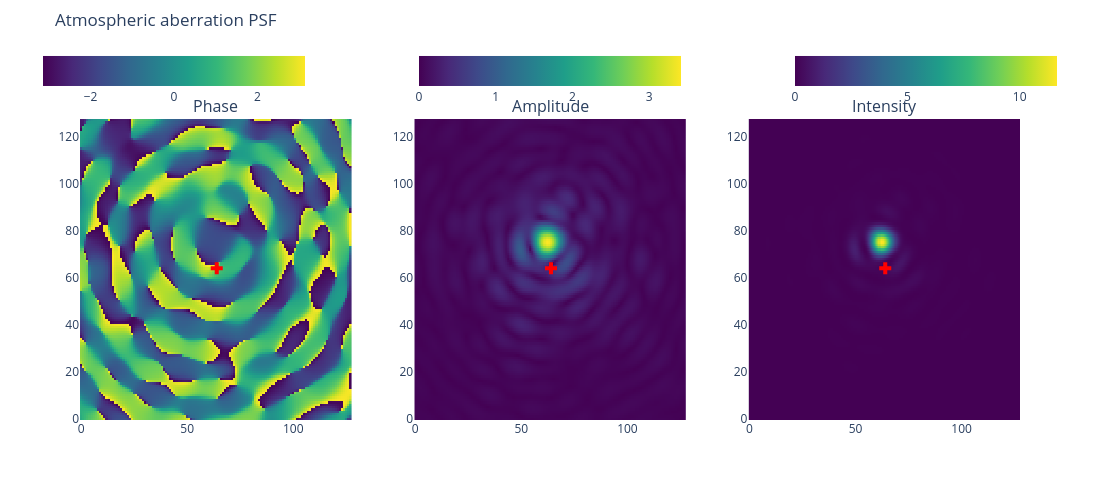
\includegraphics[width=0.4\textwidth]{pid-atmosphericaberrationpsf.png}
					\caption{Example original sized PSF}\hspace{\fill}
				\end{figure*}				
				\item \textbf{Cropped sized PSFs}:  Two datasets of 70000 electric fields and corresponding intensities stored in 64x64x2 and 64x64 matrices respectively. These cropped  PSFs correspond to the central pixels from the Original sized PSFs.
				\begin{figure*}[ht!]
					\centering
					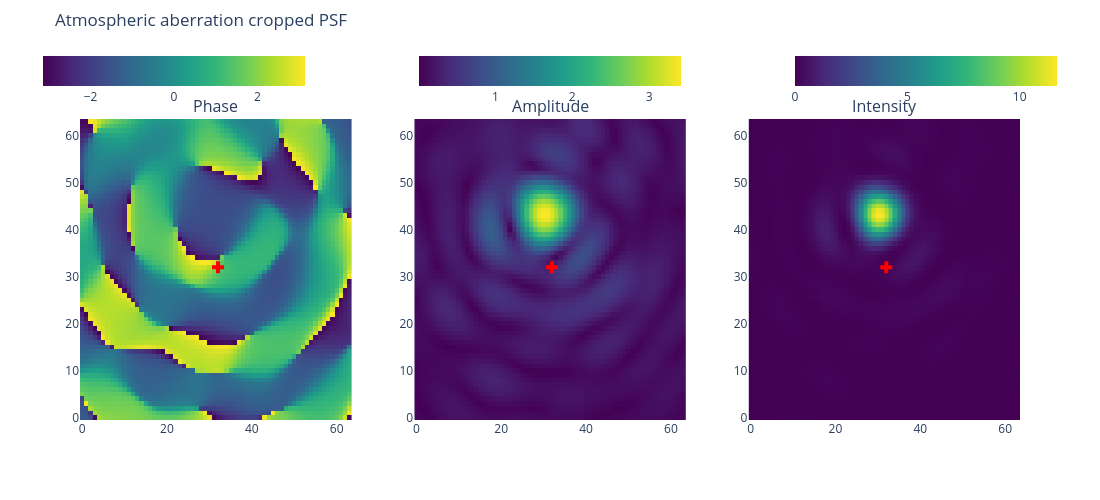
\includegraphics[width=0.4\textwidth]{pid-atmosphericaberrationcroppedpsf.png}
					\caption{Example Cropped sized PSF}\hspace{\fill}
				\end{figure*}			
				\item \textbf{Original sized predicted PSFs}:  Two datasets of 70000 predicted electric fields and predicted intensities stored in 128x128x2 and 128x128 matrices respectively. These predicted PSFs are the outputs of a model trained with the Original PSFs dataset and their corresponding PL intensities.
				\begin{figure*}[ht!]
					\centering
					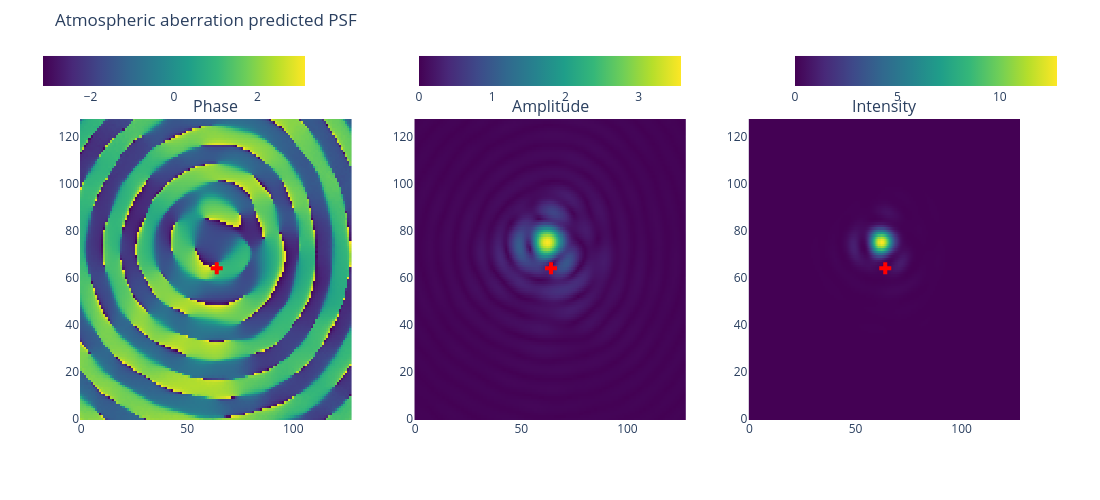
\includegraphics[width=0.4\textwidth]{pid-atmosphericaberrationpredictedpsf.png}
					\caption{Example original sized predicted PSF}\hspace{\fill}
				\end{figure*}			
				\item \textbf{Cropped sized predicted PSF}: Two datasets of 70000 predicted electric fields and predicted intensities stored in 64x64x2 and 64x64 matrices respectively. These cropped predicted PSFs are the outputs of a model trained with the Cropped sized PSFs dataset and their corresponding PL intensities (which are the same ouput intensities from the Original sized PSFs dataset).
				\begin{figure*}[ht!]
					\centering
					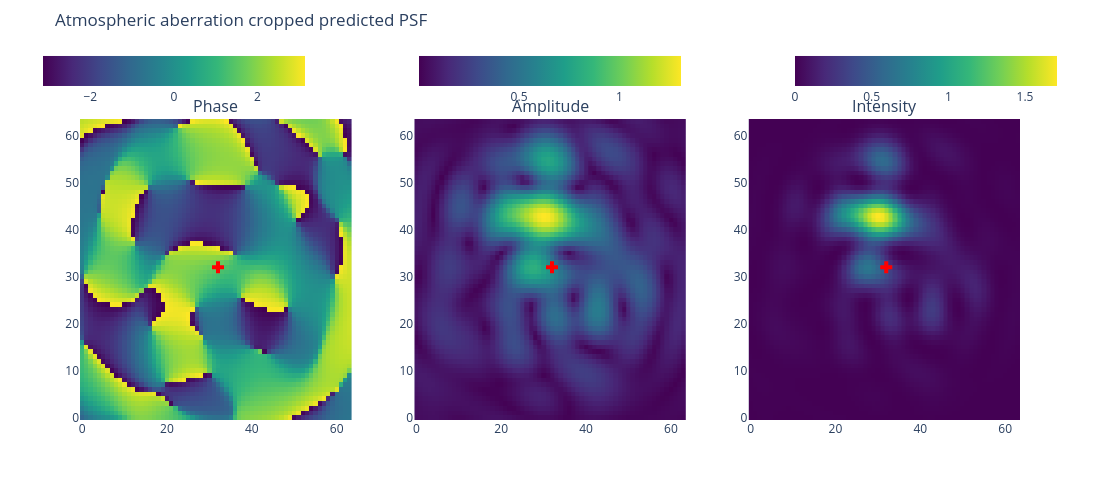
\includegraphics[width=0.4\textwidth]{pid-atmosphericaberrationcroppedpredictedpsf.png}
					\caption{Example cropped sized predicted PSF}\hspace{\fill}
				\end{figure*}
				\FloatBarrier			
			\end{itemize}
			
			
		\subparagraph{PL intensities}
		The same dataset of PL output intensities are used for every PSF dataset. The intensities are computed multiplying the LP coefficients by the transfer matrix of the \textbf{19 mode PL}. This dataset has 70000 datapoints, each datapoint being a vector of 19 elements.
		
		
	\subsubsection{Zernike modes related}
		There are 5 subgroups of datasets: PSFs generated with 2, 5, 9, 14 and 20 zernike modes. Each subgroup is divided in original sized, cropped sized, predicted and cropped predicted as in the case of the atmospheric aberration PSFs.
		
		
		\subparagraph{2 Zernike modes PSFs}
			\begin{itemize}
				\item \textbf{Original sized 2 modes PSFs}: Two datasets of 70000 electric fields and corresponding intensities stored in 128x128x2 and 128x128 matrices respectively. The aberration by a 2 modes zernike basis.		
				\item \textbf{Cropped sized 2 modes PSFs}:  Two datasets of 70000 electric fields and corresponding intensities stored in 64x64x2 and 64x64 matrices respectively. These cropped  PSFs correspond to the central pixels from the Original sized 2 modes PSFs.
				\item \textbf{Original sized predicted 2 modes PSFs}:  Two datasets of 70000 predicted electric fields and predicted intensities stored in 128x128x2 and 128x128 matrices respectively. These predicted PSFs are the outputs of a model trained with the Original sized 2 modes PSFs dataset and their corresponding PL intensities.
				\item \textbf{Cropped sized predicted 2 modes PSF}: Two datasets of 70000 predicted electric fields and predicted intensities stored in 64x64x2 and 64x64 matrices respectively. These cropped predicted PSFs are the outputs of a model trained with the Cropped sized 2 modes PSFs dataset and their corresponding PL intensities (which are the same ouput intensities from the Original sized 2 modes PSFs dataset).
			\end{itemize}
			
			\begin{figure*}[ht!]
				\centering
				\subfloat[Original sized 2 modes PSF example]{%
					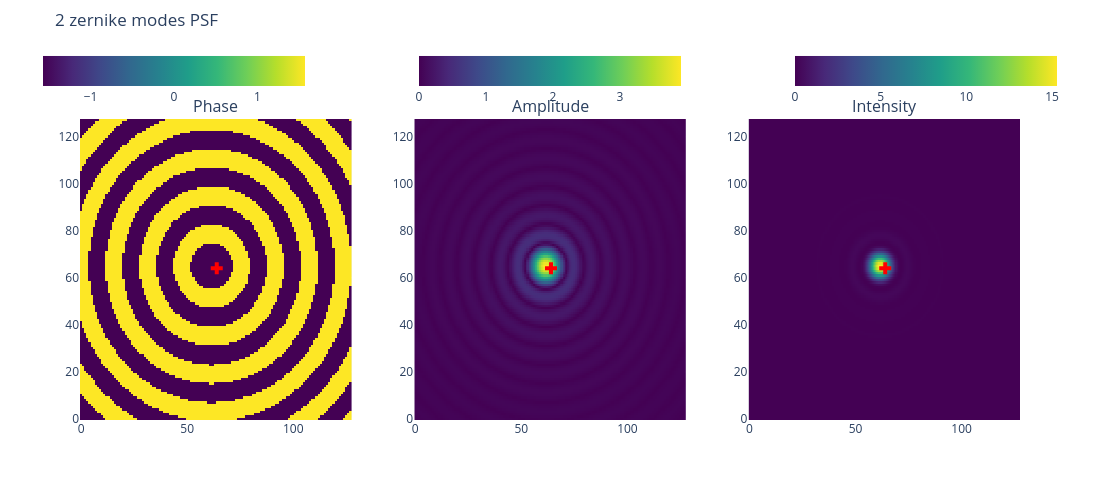
\includegraphics[width=0.6\textwidth]{pid-2zernikemodespsf.png}}\\
					
				\subfloat[Cropped sized 2 modes PSF example]{%
					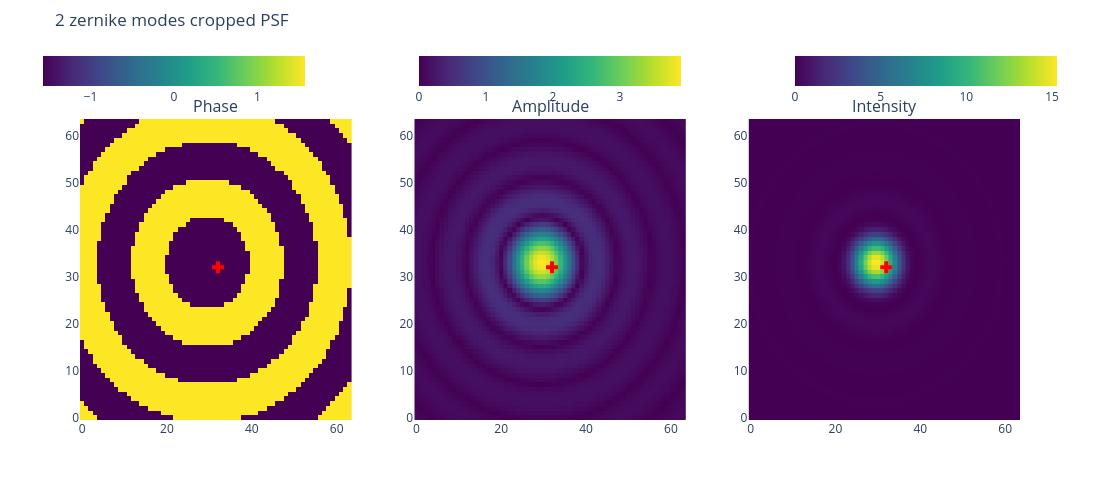
\includegraphics[width=0.6\textwidth]{pid-2zernikemodescroppedpsf}}\\
					
				\subfloat[Original sized predicted 2 modes PSF example]{%
					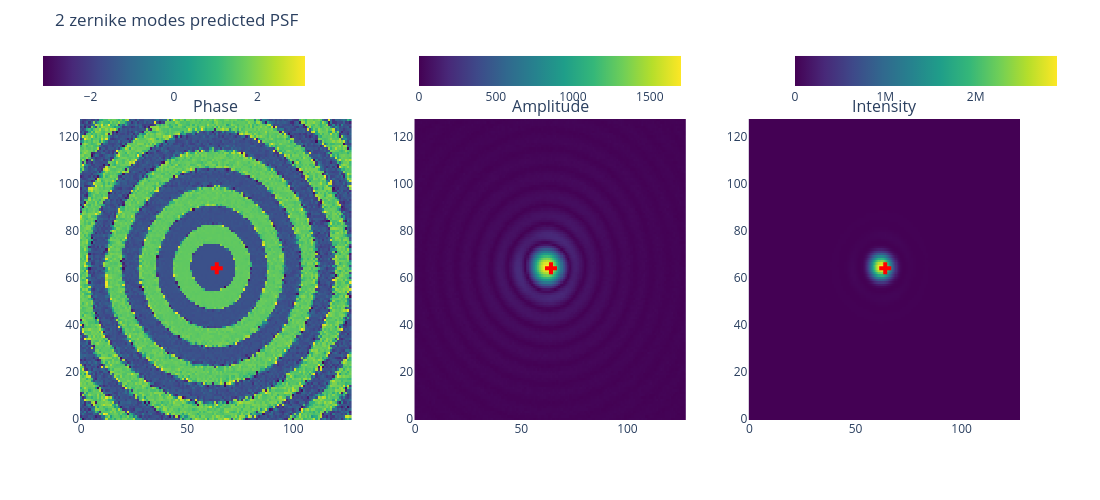
\includegraphics[width=0.6\textwidth]{pid-2zernikemodespredictedpsf}}\\
					
				\subfloat[cropped sized predicted 2 modes PSF example]{%
					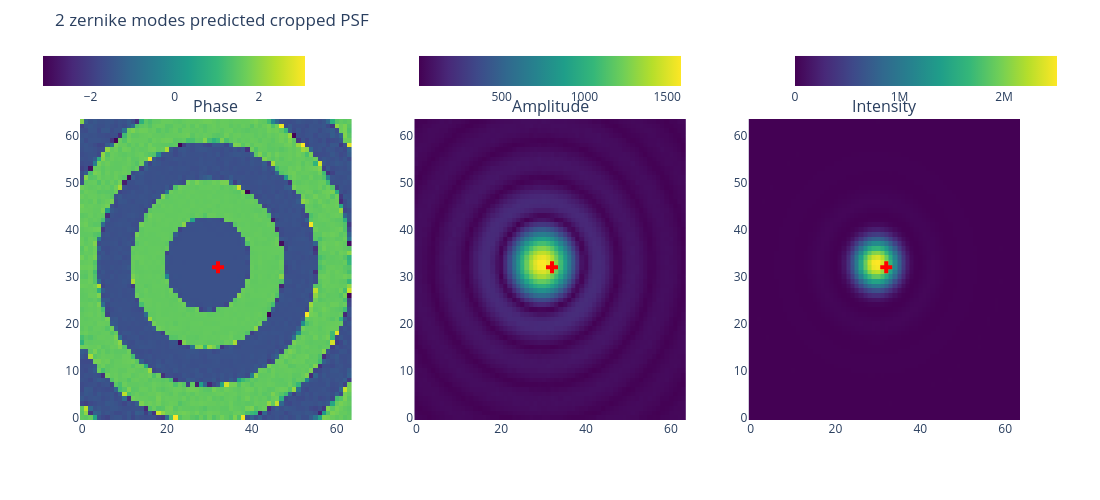
\includegraphics[width=0.6\textwidth]{pid-2zernikemodespredictedcroppedpsf}}\\
			\caption{2 Zernike modes PSF datasets examples}
		\end{figure*}
			\FloatBarrier
			
			
			\subparagraph{5 Zernike modes PSFs}
			\begin{itemize}
				\item \textbf{Original sized 5 modes PSFs}: Two datasets of 70000 electric fields and corresponding intensities stored in 128x128x2 and 128x128 matrices respectively. The aberration by a 5 modes zernike basis.		
				\item \textbf{Cropped sized 5 modes PSFs}:  Two datasets of 70000 electric fields and corresponding intensities stored in 64x64x2 and 64x64 matrices respectively. These cropped  PSFs correspond to the central pixels from the Original sized 5 modes PSFs.
				\item \textbf{Original sized predicted 5 modes PSFs}:  Two datasets of 70000 predicted electric fields and predicted intensities stored in 128x128x2 and 128x128 matrices respectively. These predicted PSFs are the outputs of a model trained with the Original sized 5 modes PSFs dataset and their corresponding PL intensities.	
				\item \textbf{Cropped sized predicted 5 modes PSF}: Two datasets of 70000 predicted electric fields and predicted intensities stored in 64x64x2 and 64x64 matrices respectively. These cropped predicted PSFs are the outputs of a model trained with the Cropped sized 5 modes PSFs dataset and their corresponding PL intensities (which are the same ouput intensities from the Original sized 5 modes PSFs dataset).
			\end{itemize}
			
			\begin{figure*}[ht!]
				\centering
				\subfloat[Original sized 5 modes PSF example]{%
					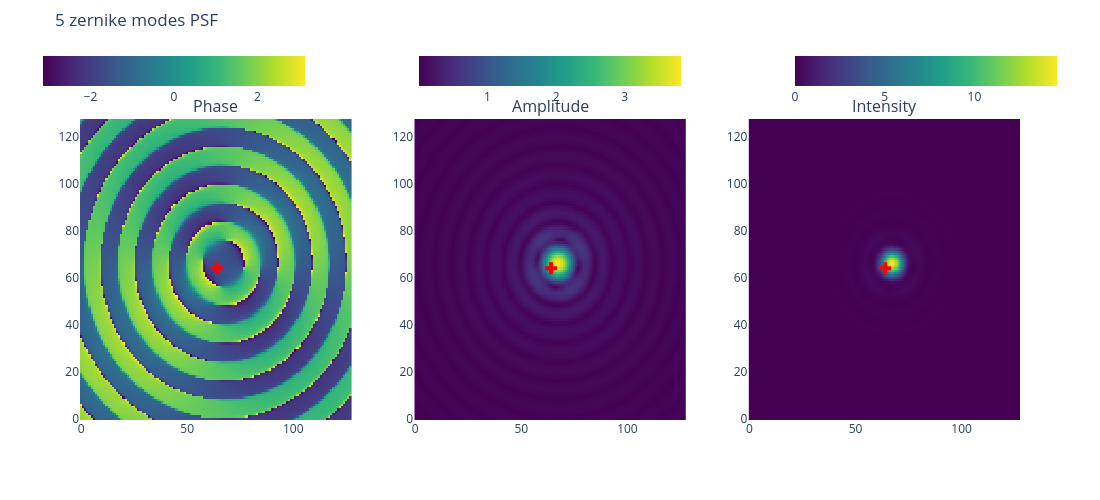
\includegraphics[width=0.6\textwidth]{pid-5zernikemodespsf.png}}\\
					
				\subfloat[Cropped sized 5 modes PSF example]{%
					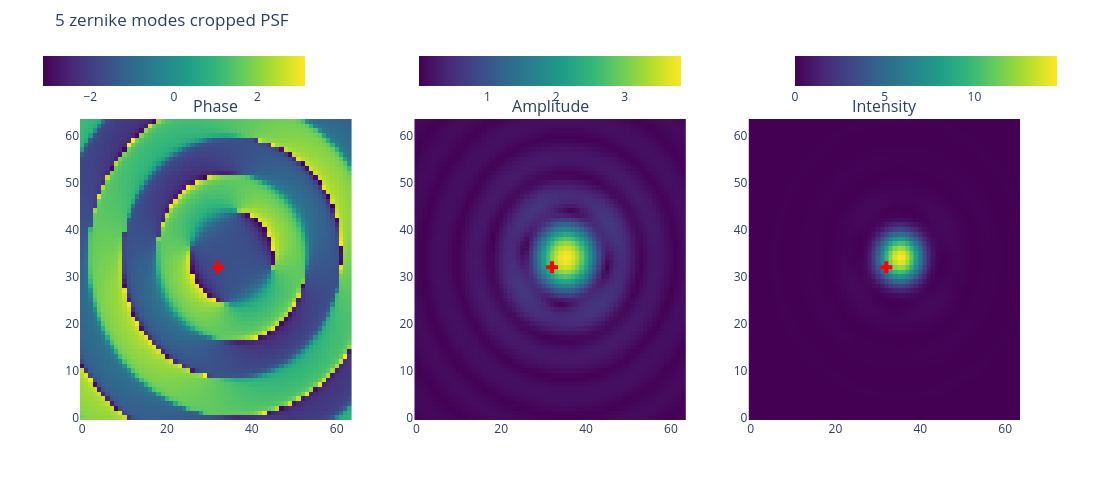
\includegraphics[width=0.6\textwidth]{pid-5zernikemodescroppedpsf}}\\
					
				\subfloat[Original sized predicted 5 modes PSF example]{%
					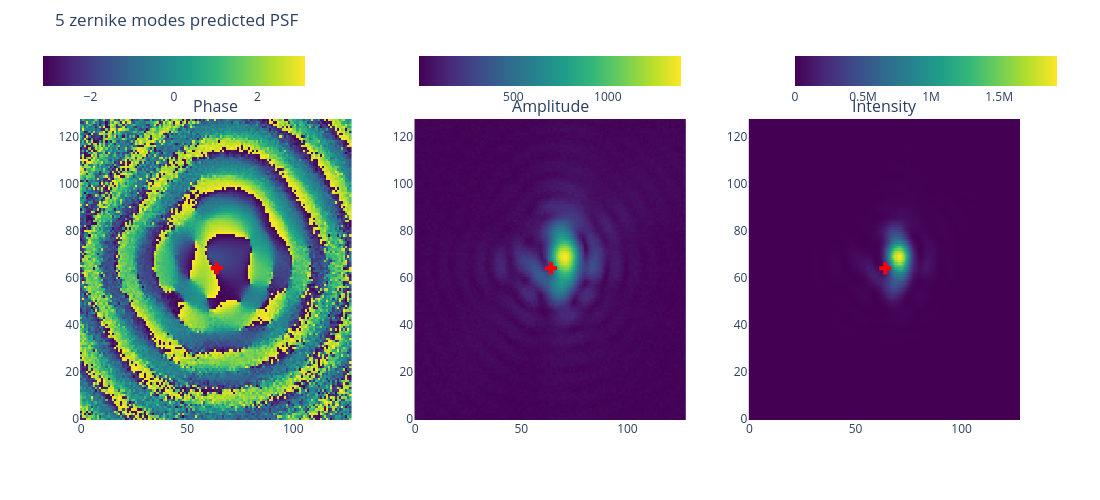
\includegraphics[width=0.6\textwidth]{pid-5zernikemodespredictedpsf}}\\
					
				\subfloat[cropped sized predicted 5 modes PSF example]{%
					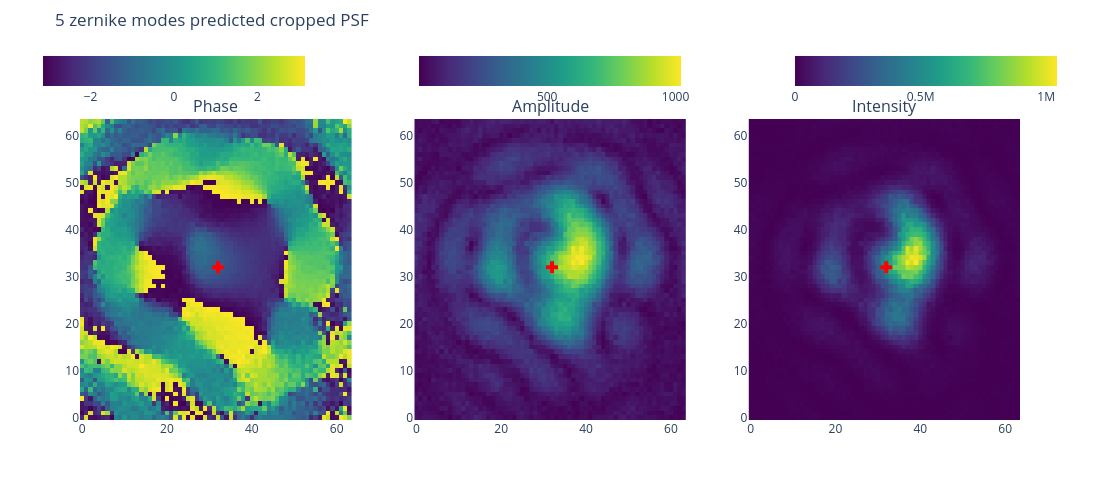
\includegraphics[width=0.6\textwidth]{pid-5zernikemodespredictedcroppedpsf}}\\
			
			\caption{5 Zernike modes PSF datasets examples}
		\end{figure*}
			\FloatBarrier
			
			
			\subparagraph{9 Zernike modes PSFs}
			\begin{itemize}
				
				\item \textbf{Original sized 9 modes PSFs}: Two datasets of 70000 electric fields and corresponding intensities stored in 128x128x2 and 128x128 matrices respectively. The aberration by a 9 modes zernike basis.		
				\item \textbf{Cropped sized 9 modes PSFs}:  Two datasets of 70000 electric fields and corresponding intensities stored in 64x64x2 and 64x64 matrices respectively. These cropped  PSFs correspond to the central pixels from the Original sized 9 modes PSFs.
				\item \textbf{Original sized predicted 9 modes PSFs}:  Two datasets of 70000 predicted electric fields and predicted intensities stored in 128x128x2 and 128x128 matrices respectively. These predicted PSFs are the outputs of a model trained with the Original sized 9 modes PSFs dataset and their corresponding PL intensities.
				\item \textbf{Cropped sized predicted 9 modes PSF}: Two datasets of 70000 predicted electric fields and predicted intensities stored in 64x64x2 and 64x64 matrices respectively. These cropped predicted PSFs are the outputs of a model trained with the Cropped sized 9 modes PSFs dataset and their corresponding PL intensities (which are the same ouput intensities from the Original sized 9 modes PSFs dataset).
			\end{itemize}
			
			\begin{figure*}[ht!]
				\centering
				\subfloat[Original sized 9 modes PSF example]{%
					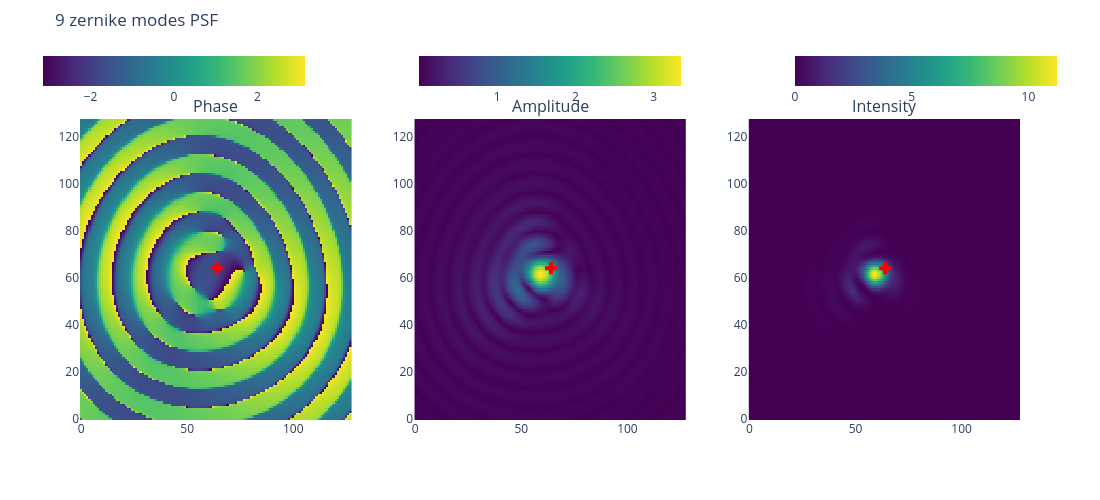
\includegraphics[width=0.6\textwidth]{pid-9zernikemodespsf.png}}\\
					
				\subfloat[Cropped sized 9 modes PSF example]{%
					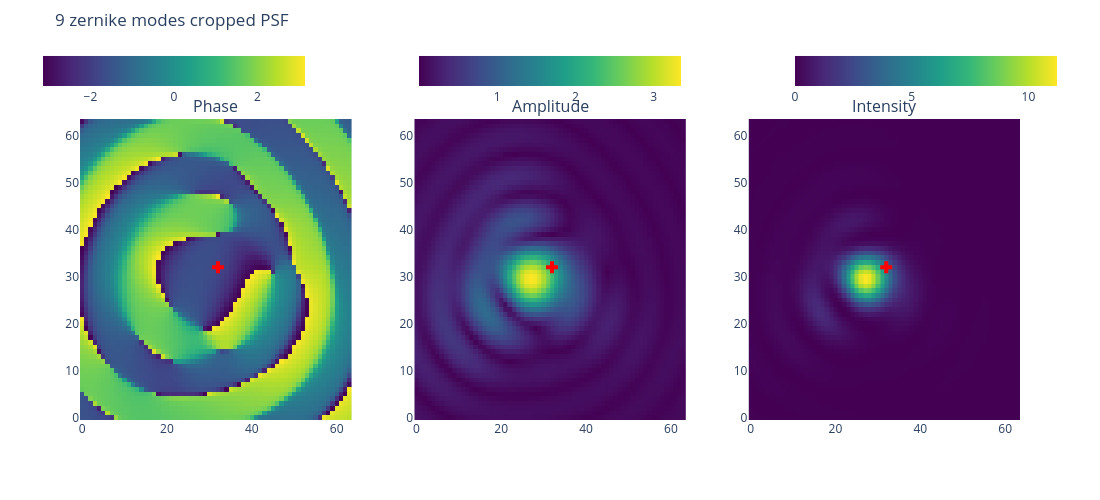
\includegraphics[width=0.6\textwidth]{pid-9zernikemodescroppedpsf}}\\
					
				\subfloat[Original sized predicted 9 modes PSF example]{%
					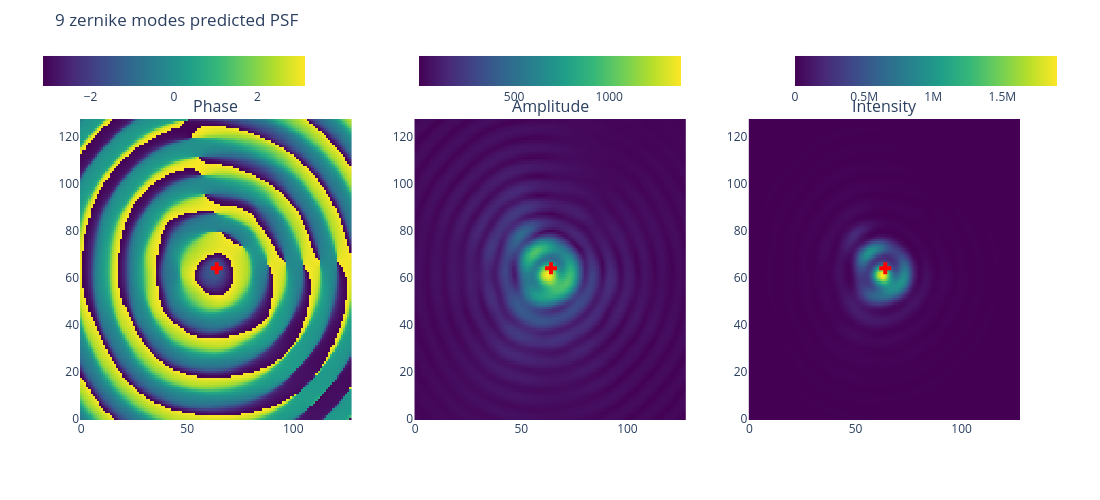
\includegraphics[width=0.6\textwidth]{pid-9zernikemodespredictedpsf}}\\
					
				\subfloat[cropped sized predicted 9 modes PSF example]{%
					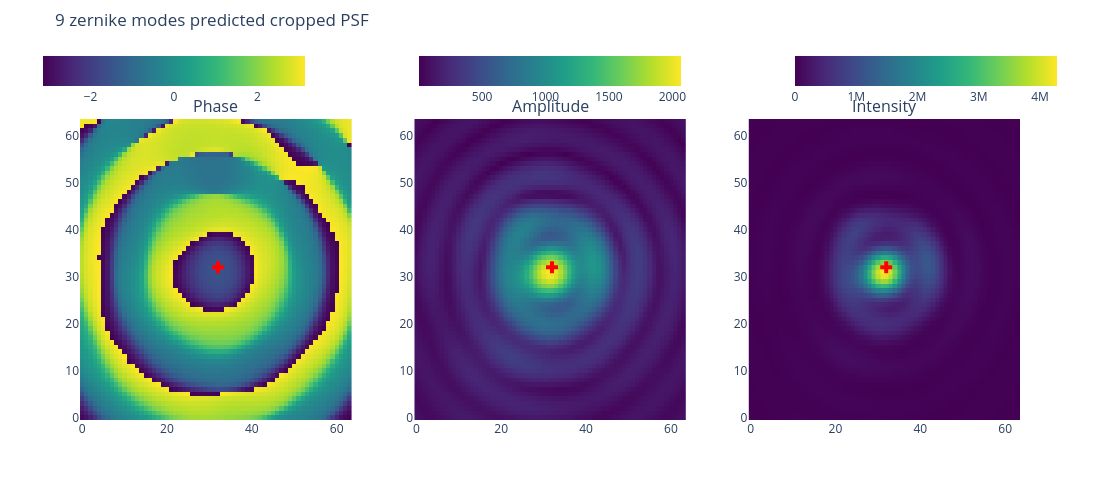
\includegraphics[width=0.6\textwidth]{pid-9zernikemodespredictedcroppedpsf}}\\
			
			\caption{9 Zernike modes PSF datasets examples}
		\end{figure*}
			\FloatBarrier
			
			
			\subparagraph{14 Zernike modes PSFs}
			\begin{itemize}
				\item \textbf{Original sized 14 modes PSFs}: Two datasets of 70000 electric fields and corresponding intensities stored in 128x128x2 and 128x128 matrices respectively. The aberration by a 14 modes zernike basis.
				\item \textbf{Cropped sized 14 modes PSFs}:  Two datasets of 70000 electric fields and corresponding intensities stored in 64x64x2 and 64x64 matrices respectively. These cropped  PSFs correspond to the central pixels from the Original sized 14 modes PSFs.
				\item \textbf{Original sized predicted 14 modes PSFs}:  Two datasets of 70000 predicted electric fields and predicted intensities stored in 128x128x2 and 128x128 matrices respectively. These predicted PSFs are the outputs of a model trained with the Original sized 14 modes PSFs dataset and their corresponding PL intensities.
				\item \textbf{Cropped sized predicted 14 modes PSF}: Two datasets of 70000 predicted electric fields and predicted intensities stored in 64x64x2 and 64x64 matrices respectively. These cropped predicted PSFs are the outputs of a model trained with the Cropped sized 14 modes PSFs dataset and their corresponding PL intensities (which are the same ouput intensities from the Original sized 14 modes PSFs dataset).
			\end{itemize}
			
			\begin{figure*}[ht!]
				\centering
				\subfloat[Original sized 14 modes PSF example]{%
					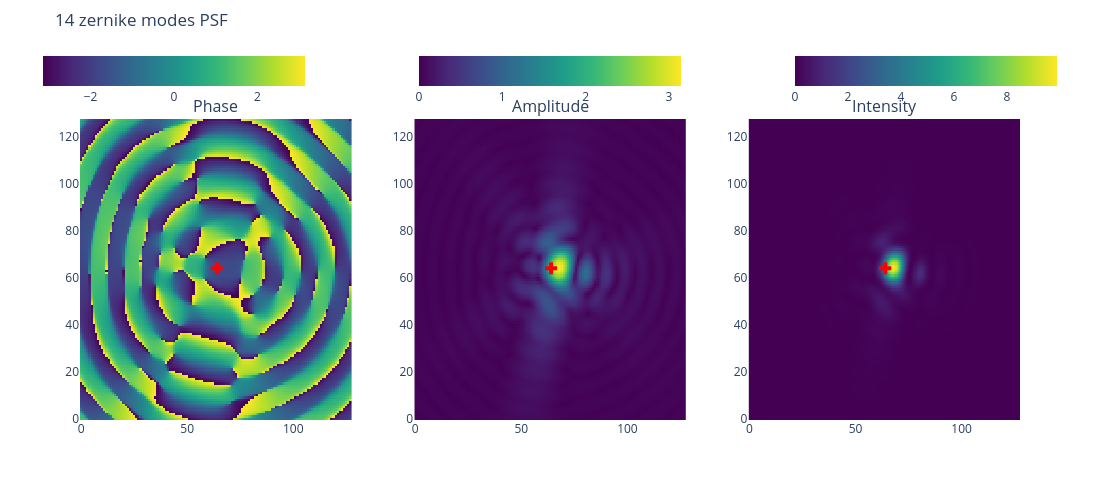
\includegraphics[width=0.6\textwidth]{pid-14zernikemodespsf.png}}\\
					
				\subfloat[Cropped sized 14 modes PSF example]{%
					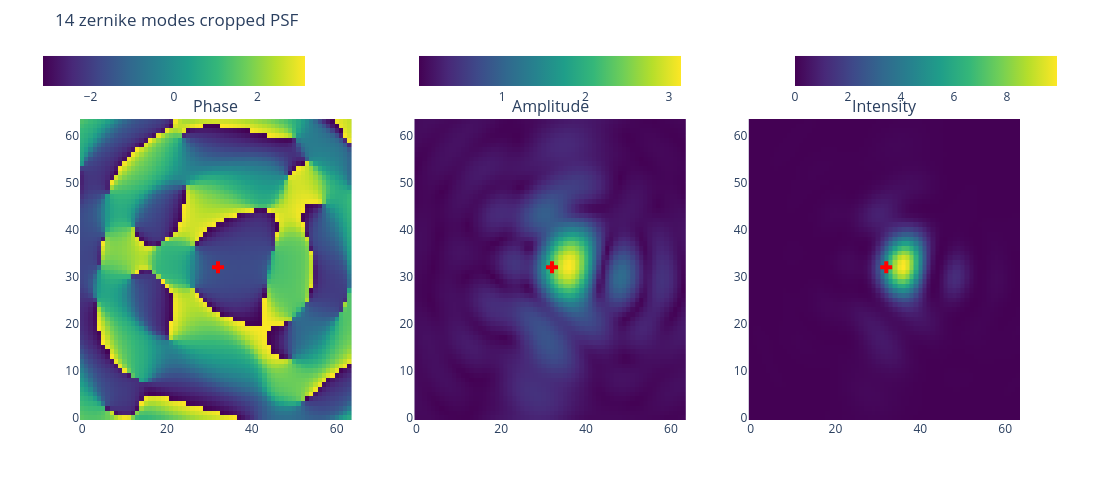
\includegraphics[width=0.6\textwidth]{pid-14zernikemodescroppedpsf}}\\
					
				\subfloat[Original sized predicted 14 modes PSF example]{%
					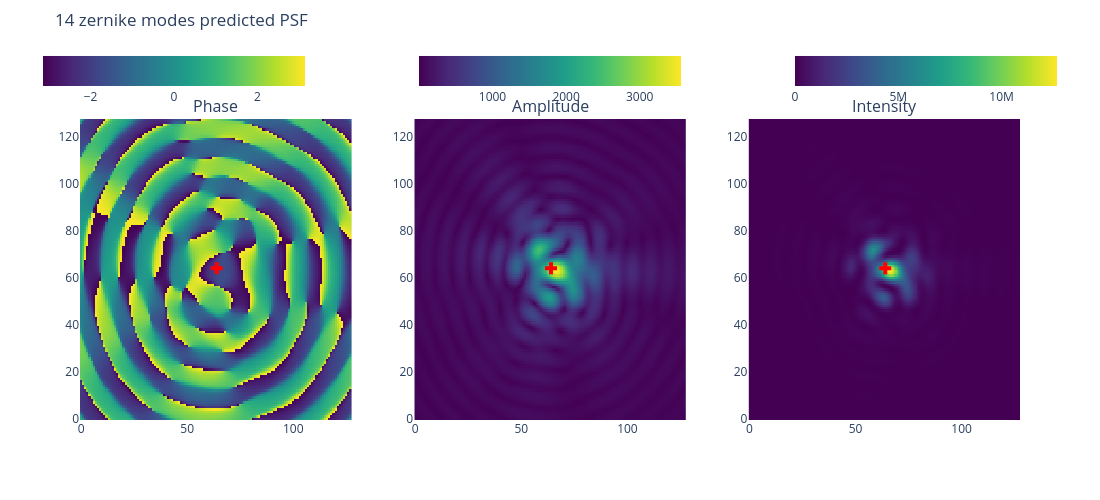
\includegraphics[width=0.6\textwidth]{pid-14zernikemodespredictedpsf}}\\
					
				\subfloat[cropped sized predicted 14 modes PSF example]{%
					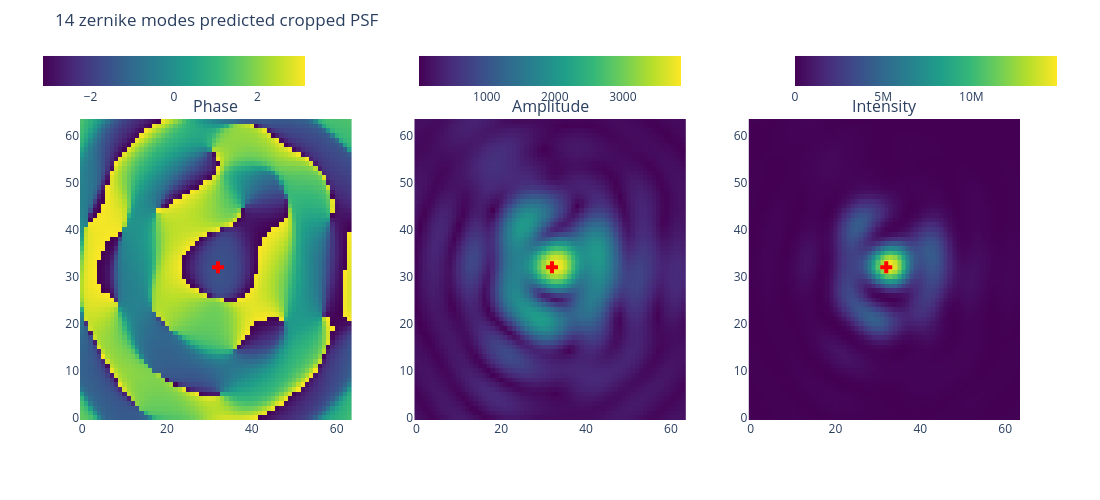
\includegraphics[width=0.6\textwidth]{pid-14zernikemodespredictedcroppedpsf}}\\
			
			\caption{14 Zernike modes PSF datasets examples}
		\end{figure*}
			\FloatBarrier
			
			
			\subparagraph{20 Zernike modes PSFs}
			\begin{itemize}
				
				\item \textbf{Original sized 20 modes PSFs}: Two datasets of 70000 electric fields and corresponding intensities stored in 128x128x2 and 128x128 matrices respectively. The aberration by a 20 modes zernike basis.			
				\item \textbf{Cropped sized 20 modes PSFs}:  Two datasets of 70000 electric fields and corresponding intensities stored in 64x64x2 and 64x64 matrices respectively. These cropped  PSFs correspond to the central pixels from the Original sized 20 modes PSFs.
				\item \textbf{Original sized predicted 20 modes PSFs}:  Two datasets of 70000 predicted electric fields and predicted intensities stored in 128x128x2 and 128x128 matrices respectively. These predicted PSFs are the outputs of a model trained with the Original sized 20 modes PSFs dataset and their corresponding PL intensities.
				\item \textbf{Cropped sized predicted 20 modes PSF}: Two datasets of 70000 predicted electric fields and predicted intensities stored in 64x64x2 and 64x64 matrices respectively. These cropped predicted PSFs are the outputs of a model trained with the Cropped sized 20 modes PSFs dataset and their corresponding PL intensities (which are the same ouput intensities from the Original sized 20 modes PSFs dataset).
			\end{itemize}
			
			\begin{figure*}[ht!]
				\centering	
				\subfloat[Original sized 20 modes PSF example]{%
					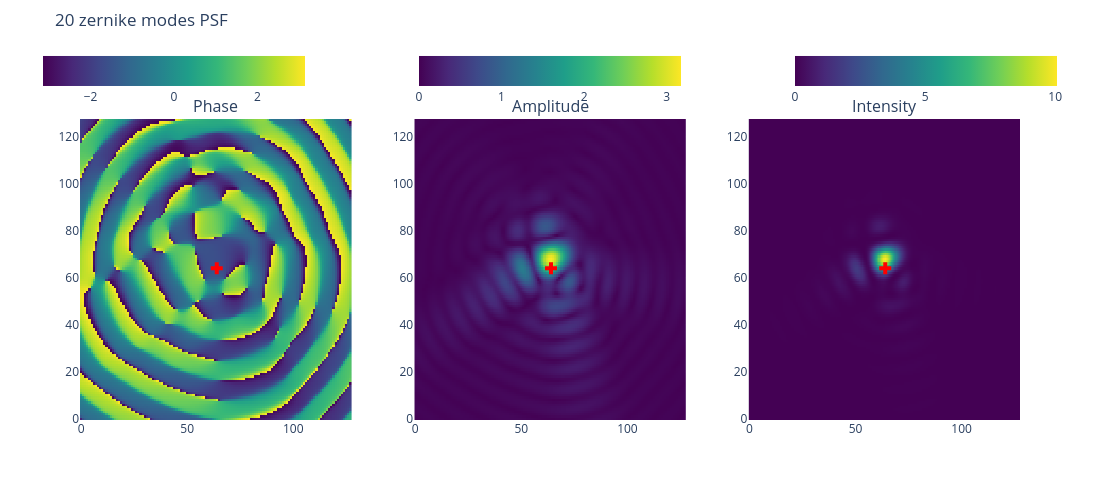
\includegraphics[width=0.6\textwidth]{pid-20zernikemodespsf.png}}\\
					
				\subfloat[Cropped sized 20 modes PSF example]{%
					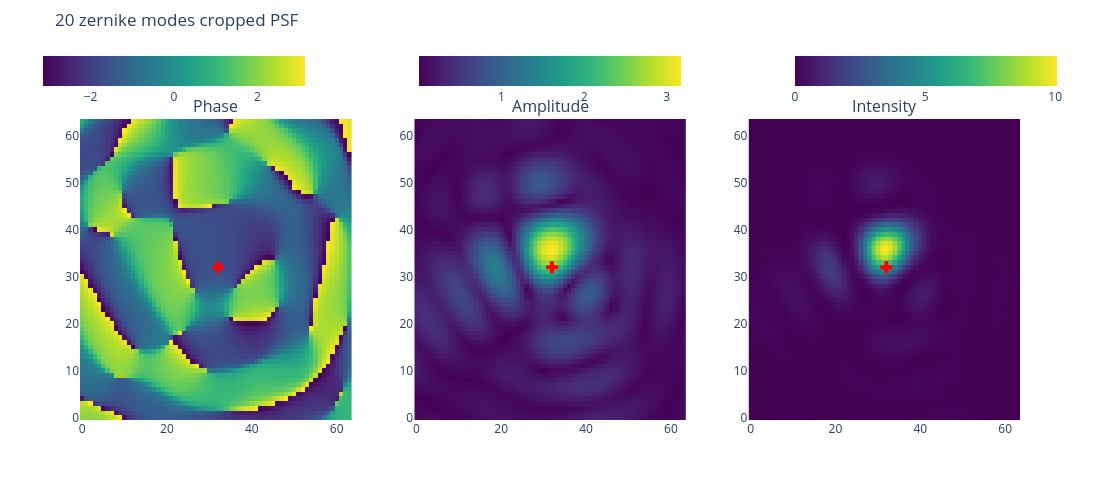
\includegraphics[width=0.6\textwidth]{pid-20zernikemodescroppedpsf}}\\
					
				\subfloat[Original sized predicted 20 modes PSF example]{%
					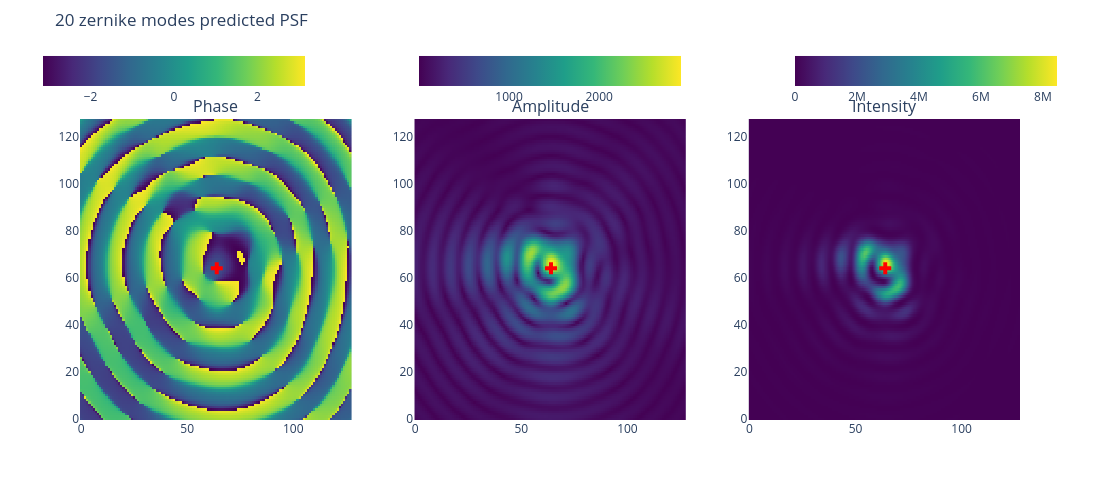
\includegraphics[width=0.6\textwidth]{pid-20zernikemodespredictedpsf}}\\
					
				\subfloat[cropped sized predicted 20 modes PSF example]{%
					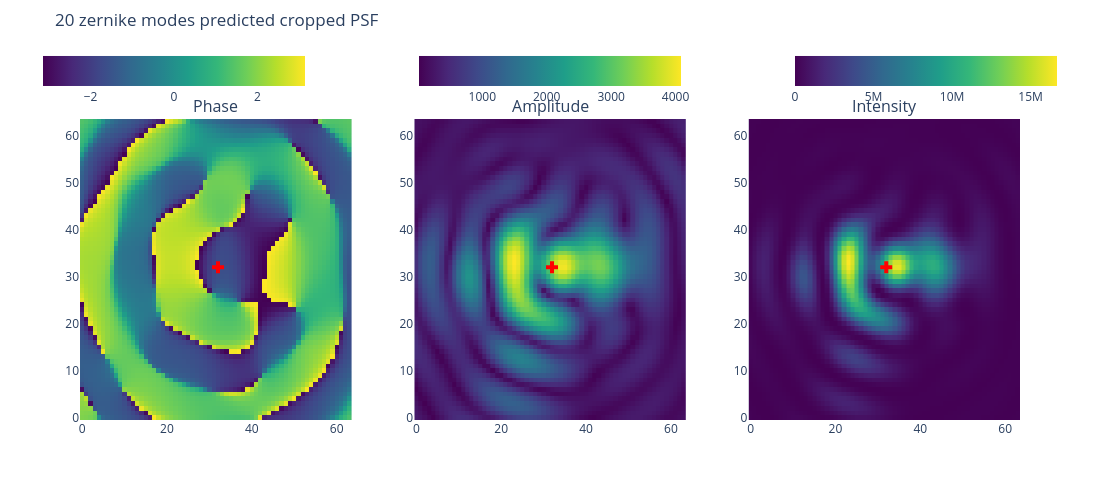
\includegraphics[width=0.6\textwidth]{pid-20zernikemodespredictedcroppedpsf}}\\
			
			\caption{20 Zernike modes PSF datasets examples}
		\end{figure*}
		\FloatBarrier
		\subparagraph{LP mode coefficients}
			There are two PL intensities dataset per Zernike aberration PSF subgroup: LP modes coefficients for 2, 5, 9, 14, 20 modes PSFs. Each of the dataset has 70000 datapoints each datapoint being the complex coefficients stored in a 19x2 matrix that separates the real and imaginary part of the coefficients.\\
			
			The two datasets correspond to the LP coefficients that are computed in the multimode end of Photonic Lanterns. The PLs are:
			\begin{itemize}
				\item 19 mode supporting multimode end with 19 waveguides in the single mode end.
				\item 42 mode supporting multimode end with 42 waveguides in the single mode end.
			\end{itemize}
			
		\subparagraph{PL intensities}
		
			There is one PL intensities dataset per Zernike aberration PSF subgroup: PL intensities for 2, 5, 9, 14, 20 modes PSFs. Each of the dataset has 70000 datapoints each datapoint being the 19 intensities corresponding to the PSF
			
			The two datasets correspond to the single mode end intensities of Photonic Lanterns. The PLs are:
			\begin{itemize}
				\item 19 mode supporting multimode end with 19 waveguides in the single mode end.
				\item 42 mode supporting multimode end with 42 waveguides in the single mode end.
			\end{itemize}

\finishday